\section{Method}

This chapter is structured around the project's three-pronged approach, directly answering the defined Sub-Research Questions (SRQs):

\begin{enumerate}
\item \textbf{Data Infrastructure (SRQ1):} The development of the Dataset Construction Engine (DCE). This section details how a custom software architecture was engineered to bypass manual annotation bottlenecks and streamline dataset creation.
\item \textbf{Dataset Creation \& Model Evaluation (SRQ2):} The practical application of the DCE to construct the \textit{UAVape} dataset—a tailored, UAV-oriented micro-litter dataset specific to UK urban environments. This section also covers how this data was rigorously evaluated through data-centric ablations on modern YOLO architectures to maximize detection performance.
\item \textbf{Operational Translation (SRQ3):} The translation of raw YOLO bounding-box detections into a conceptual mobile workflow prototype. This section explores how a smartphone-based UI could guide UK municipal cleaners to efficiently locate and segregate disposable vapes as hazardous electronic waste.
\end{enumerate}


\subsection{DCE Method}

\textbf{SRQ 1:} How can an integrated dataset construction engine bypass manual bottlenecks to improve the sourcing, annotation, metadata richness, and model-readiness of fragmented micro-WEEE imagery?

As established in Section 3, current commercial annotation platforms assume that users already possess a mature dataset. This does not hold for early-stage computer vision projects, where raw images must be sourced, aggregated, annotated, audited, and exported before model development can begin.

To address this gap, the Dataset Construction Engine (DCE) was developed as an end-to-end data factory for building the UAVape dataset. Rather than requiring separate tools for web sourcing, synthetic generation, annotation, review, and export, the DCE consolidates these stages into a single interface. The DCE aims to democratize the dataset creation process by explicitly targeting true user pain points: efficiency, transparency, and mechanical fatigue. 

The DCE is summarized in the following pipeline:

\begin{figure}[H]
    \centering
    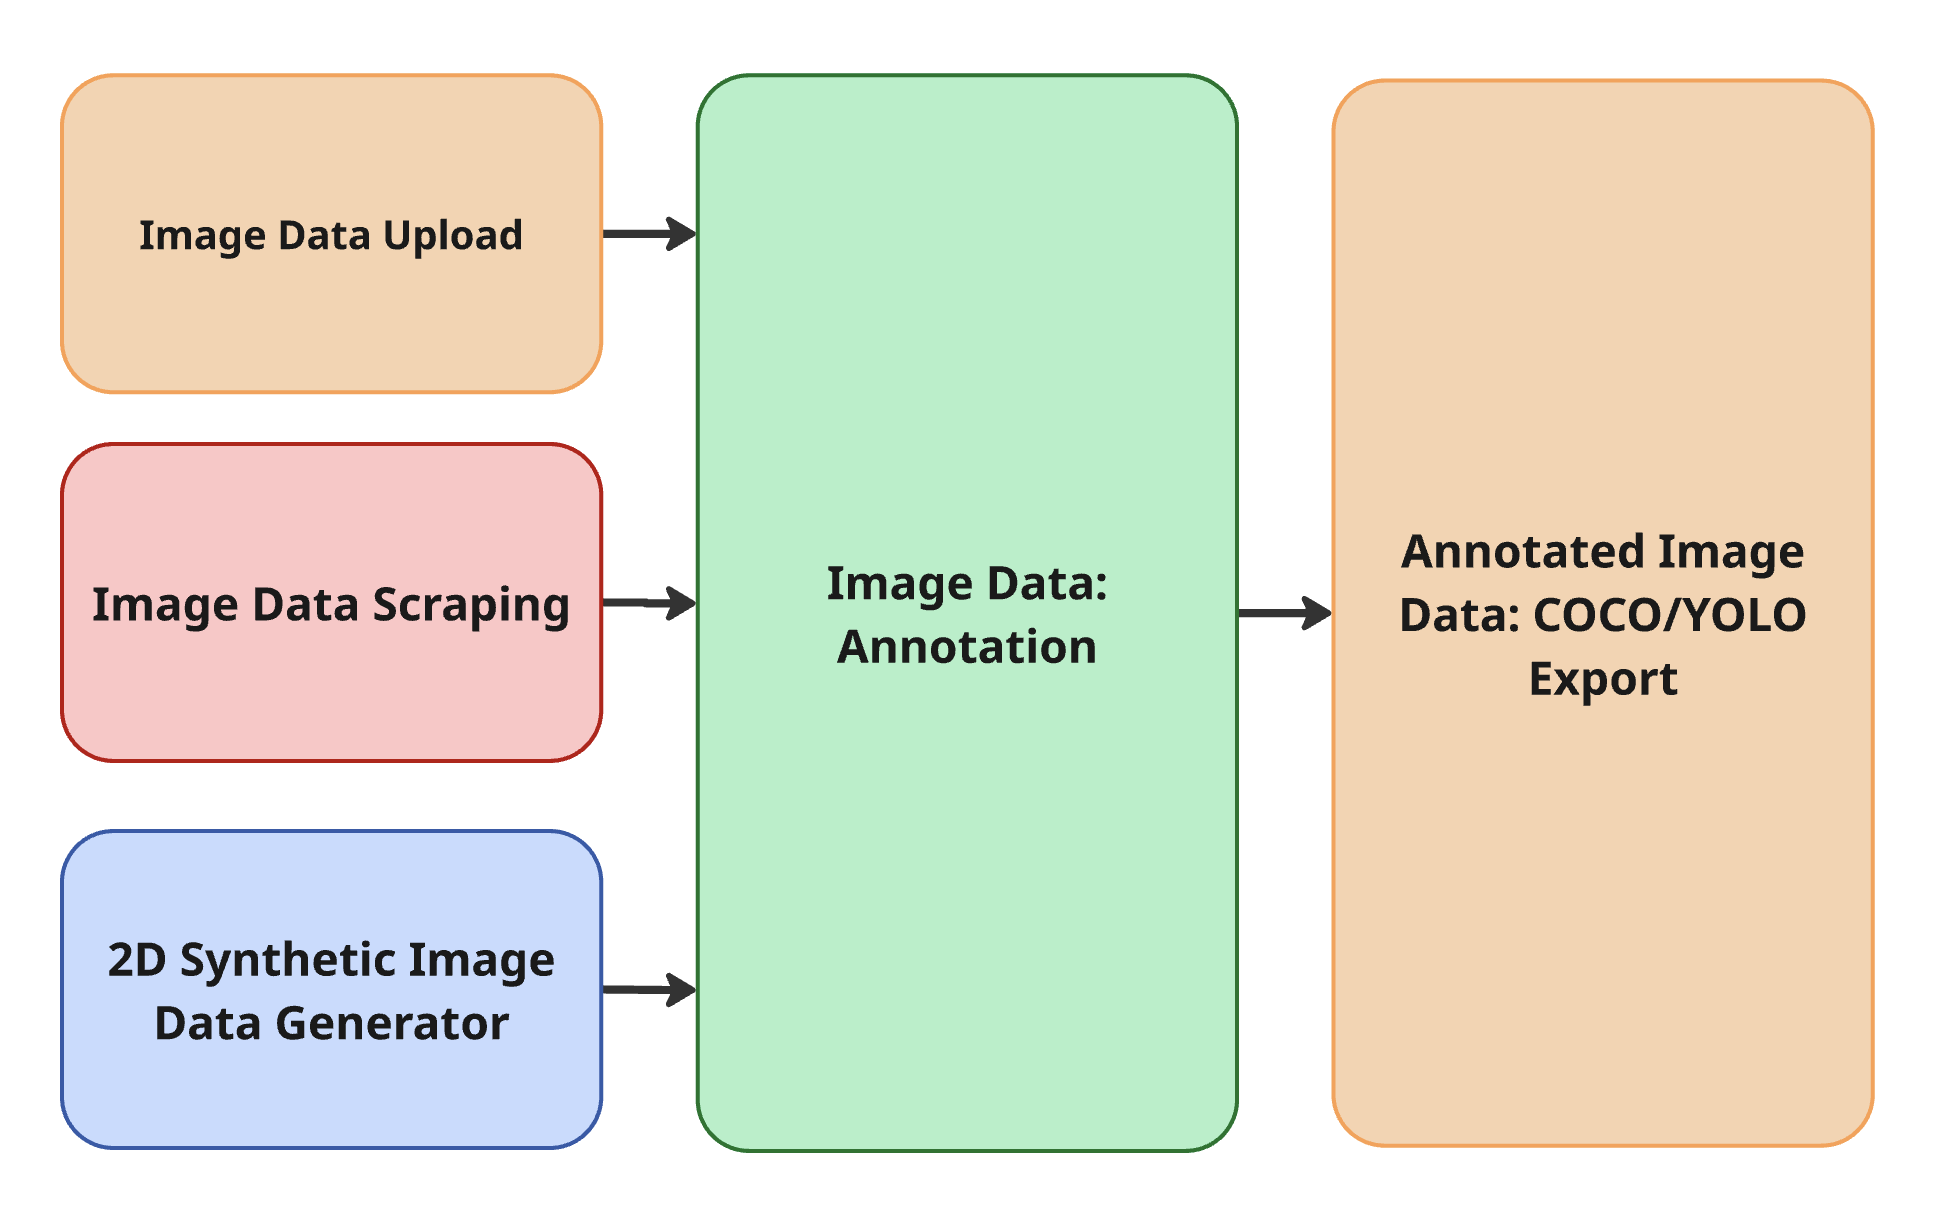
\includegraphics[width=0.4\linewidth]{DCE Abstracted.png} % Your flowchart image
    \caption{The integrated DCE workflow: from multi-source intake to YOLO export.}
    \label{fig:dce_flowchart}
\end{figure}

\subsubsection{Multi-Data Source Intake (Uploads, Video, and Scraping)}
Niche data sets, such as UAV vape litter images, may be hard to acquire on a mass scale, so the DCE aims to support diverse data streams:

\begin{itemize}
    \item \textbf{Batch Uploads:} To handle real data, the system supports high-volume batch uploading. A cryptographic hashing function was implemented at upload to automatically flag and block duplicate files.  
    \item \textbf{Integrated API Web-Scraping:} To expand the dataset and capture greater object variation, an automated scraper was built with Bing and DuckDuckGo (DDG) image APIs. Users can input exact search queries, set image limits, and utilize a ``slow-search'' delay to bypass API rate-limiting. Scraped images are automatically filtered for corrupt or unreadable files before being passed to the staging area.
    \item \textbf{Video Temporal Consolidation:} To support future drone-based use, the system also accepts \verb|.mp4| video uploads. Videos are automatically converted into image frames at user-defined time intervals, helping to capture meaningful visual differences rather than near-duplicate frames.
\end{itemize}

\textbf{Validation Benchmark:} Image uploading was validated by tracking the number of images uploaded, duplicate files detected, batch size, and the time taken to import larger batches. This allowed upload speed to be estimated as:

\begin{equation}
\label{eq:upload_speed}
U_s = \frac{N_{\text{uploaded}}}{t_{\text{upload}}}
\end{equation}

where \(U_s\) is the upload speed in images per minute, \(N_{\text{uploaded}}\) is the number of images uploaded, and \(t_{\text{upload}}\) is the upload time in minutes.

Web scraping was validated by recording the number of scrape runs completed and the number of duplicate or corrupted files detected and blocked.


\vspace{0.5em}
\noindent\textbf{$\rightarrow$ Design requirements addressed:} DCE-DR1.

\subsubsection{Synthetic Bootstrapping}
Because scraped images may not always provide enough domain-relevant context, a 2D synthetic generation module was developed. Users upload two asset types: vape cutouts and background images. The system then allows users to control scale, rotation, shadows, and colour jitter, so the vape can be composited onto the background with greater realism and visual variation.

\begin{figure}[H]
    \centering
    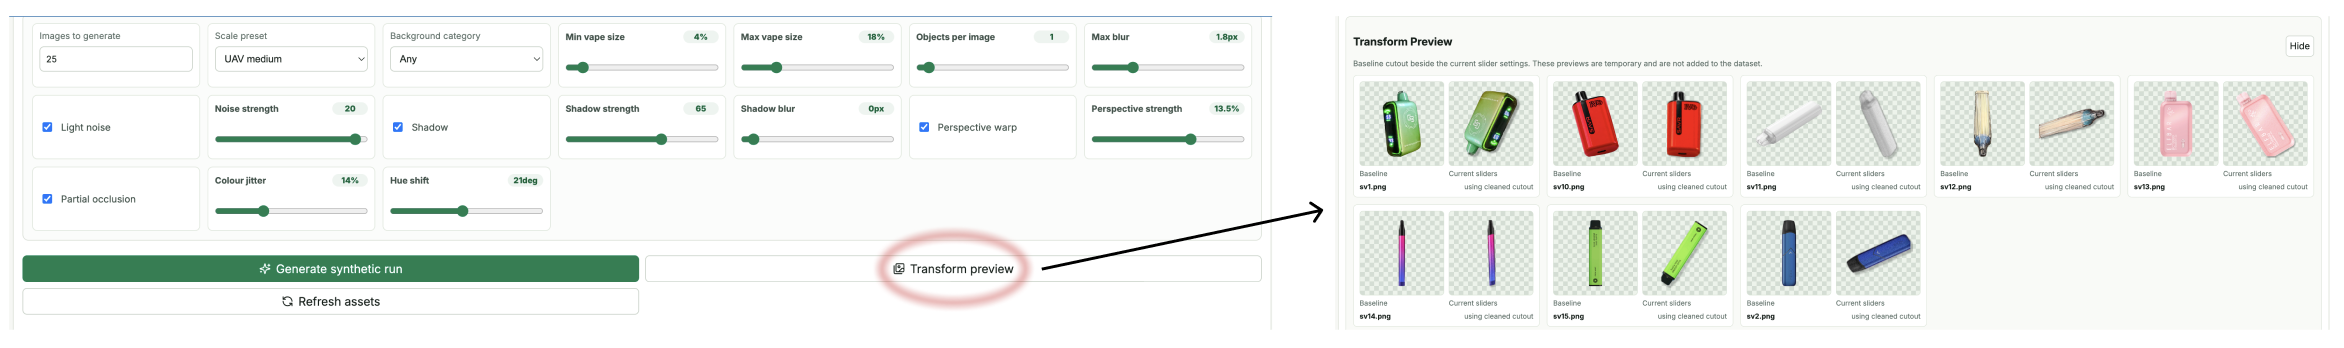
\includegraphics[width=0.9\linewidth]{synthetic panel.png}
    \caption{DCE Synthetic Vape Previews}
    \label{fig:dce_synthetic_previews}
\end{figure}

Synthetic images are saved in a separate data directory and kept separate from real-world validation images. They are only added to the main dataset when the user explicitly promotes them.

\textbf{Validation Benchmark:} This module was validated by comparing the total number of synthetic images generated with the number manually accepted by the user. This produced an acceptance rate, indicating how often the synthetic generation process created useful and visually diverse training images:

\begin{equation}
\label{eq:synthetic_acceptance_rate}
A_s = \frac{N_{\text{accepted}}}{N_{\text{generated}}} \times 100
\end{equation}

where \(A_s\) is the synthetic acceptance rate in percent, \(N_{\text{accepted}}\) is the number of manually accepted synthetic images, and \(N_{\text{generated}}\) is the total number of synthetic images generated.

\subsubsection{Human-in-the-Loop Curation (The Review Queue)}

Standard annotation tools typically focus on labelling target objects and provide limited support for sorting clean negatives or hard negatives. Giving the user the option to explicitly manage hard negative (false-positive prone) data is important for complex object detection tasks such as vape litter detection. Conversely, when a user aggregates diverse data from multiple scrape queries or bulk uploads, this also creates a messy staging pool that must be systematically sorted before the more time-consuming annotation phase begins.

To address this, the DCE implements a Review Queue as a pre-annotation audit step. Raw candidate imagery is aggregated into a single queue, where it must be explicitly classified into one of four categories: \textit{positives}, \textit{hard negatives}, \textit{clean negatives}, or \textit{rejects}.

To improve efficiency during this triage process, the interface avoids slow drag-and-click labelling. When sorting image-by-image, users can use a dedicated hotkey layout to categorize images without moving the cursor: \texttt{U} for positives, \texttt{I} for hard negatives, \texttt{O} for clean negatives, and \texttt{P} for rejects. Alternatively, if a user imports a uniform batch of data, such as a folder of known positive drone captures, the system supports batch tagging. This allows a single classification to be applied to the full batch, avoiding unnecessary manual iteration.

\textbf{Validation Benchmark:} This module was validated by evaluating the efficiency of the hotkey and batch-tagging workflow. Mean curation throughput was calculated as:

\begin{equation}
\label{eq:curation_throughput}
C_t = \frac{N_{\text{reviewed}}}{t_{\text{session}}}
\end{equation}

where \(C_t\) is the curation throughput in images per minute, \(N_{\text{reviewed}}\) is the total number of raw images classified, and \(t_{\text{session}}\) is the active time spent in the review session.

\vspace{0.5em}
\noindent\textbf{$\rightarrow$ Design requirements addressed:} DCE-DR3.

\subsubsection{Human-Audited SAM2 Annotation}

Disposable vapes are small, slender, and often diagonal in the frame, so loose bounding boxes can include large amounts of background texture around the object. This matters because the model may learn background correlations that reduce generalisation. However, manually tracing high-quality masks across hundreds of images is slow, inconsistent and introduces potential human bias if rushed.

To reduce this burden, the DCE integrated Meta's Segment Anything Model 2 (SAM2) as an annotation assistant. SAM2 is a foundation segmentation model that can generate an object mask from a user prompt, such as a click on the target object \cite{ravi2024sam2}. In the DCE, SAM2 was used only as a proposal mechanism: every generated mask still required manual review before it could enter the dataset.

\begin{figure}[H]
    \centering
    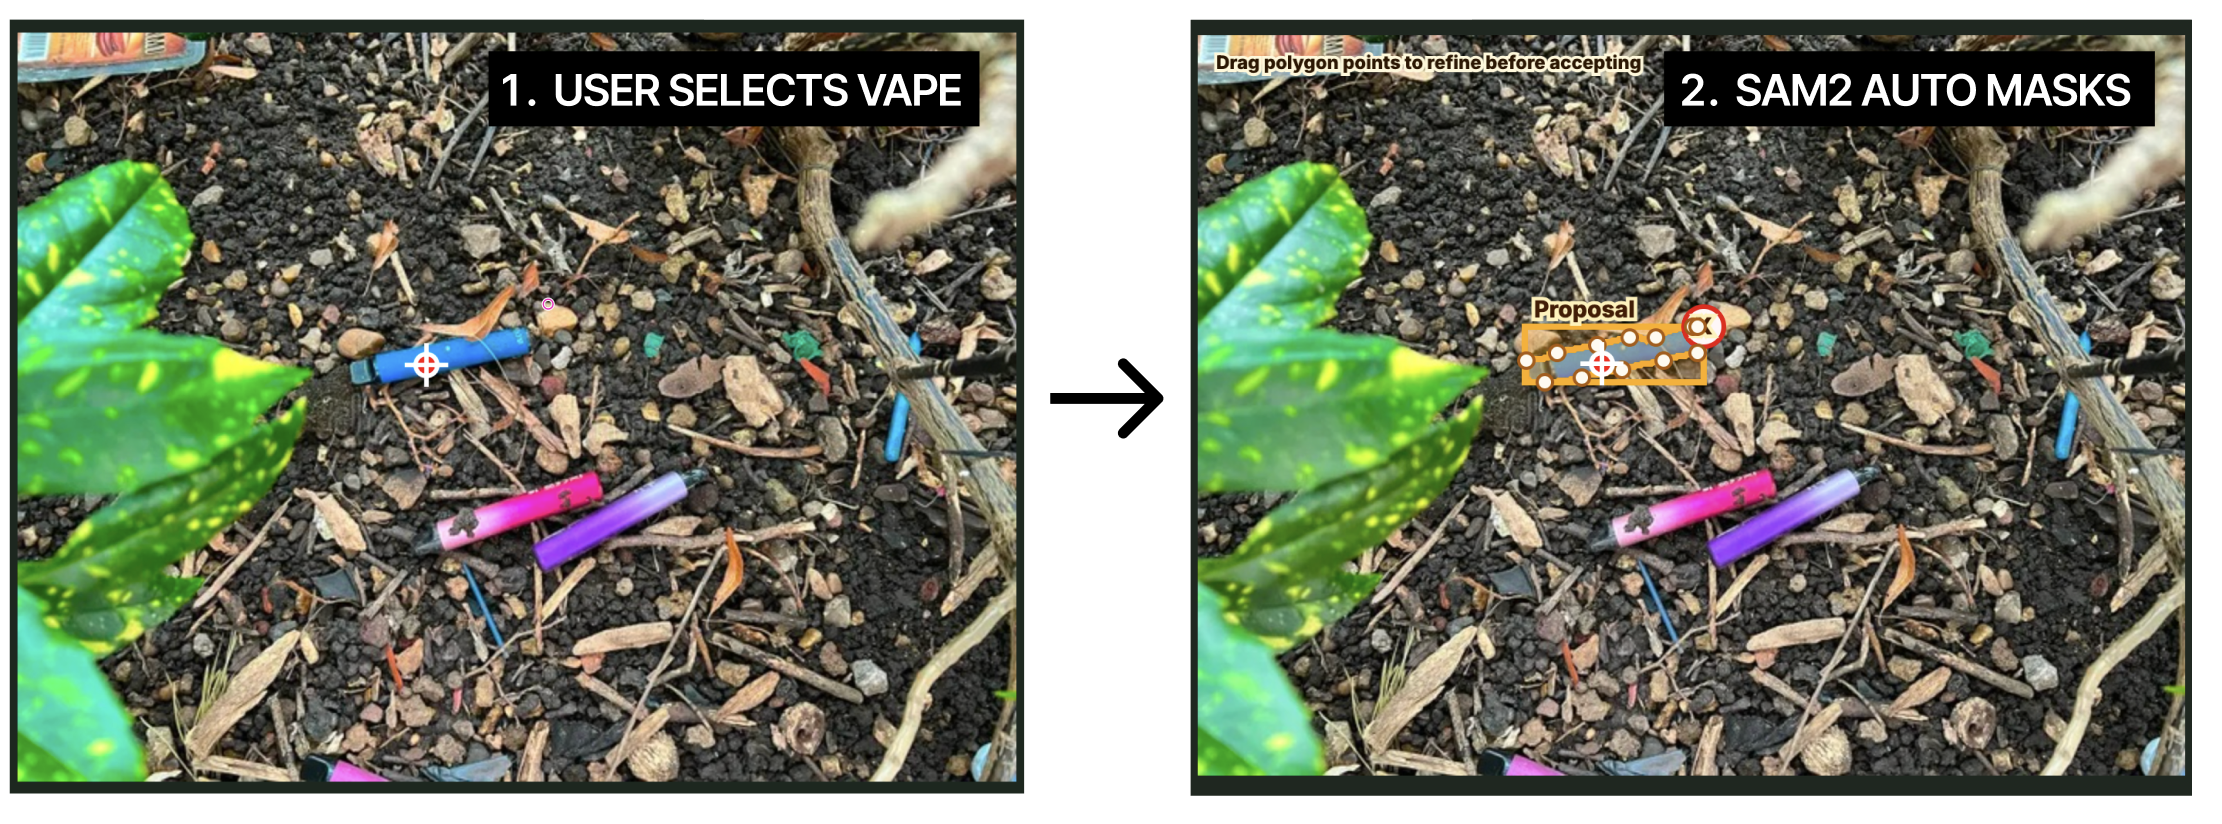
\includegraphics[width=0.5\linewidth]{SAM2 Demonstration.png}
    \caption{SAM2 Annotation Demonstration}
    \label{fig:sam2_annotation_demo}
\end{figure}

The DCE implemented this as a dedicated SAM2 Mode for batch annotation. The workflow was intentionally simple: click the object to request a mask, press Enter to accept it, re-click if the proposal is poor, and move to the next unannotated image. This reduces repeated cursor movement and speeds up large annotation sessions. Poor proposals could be cleared, corrected or deleted.

\begin{figure}[H]
    \centering
    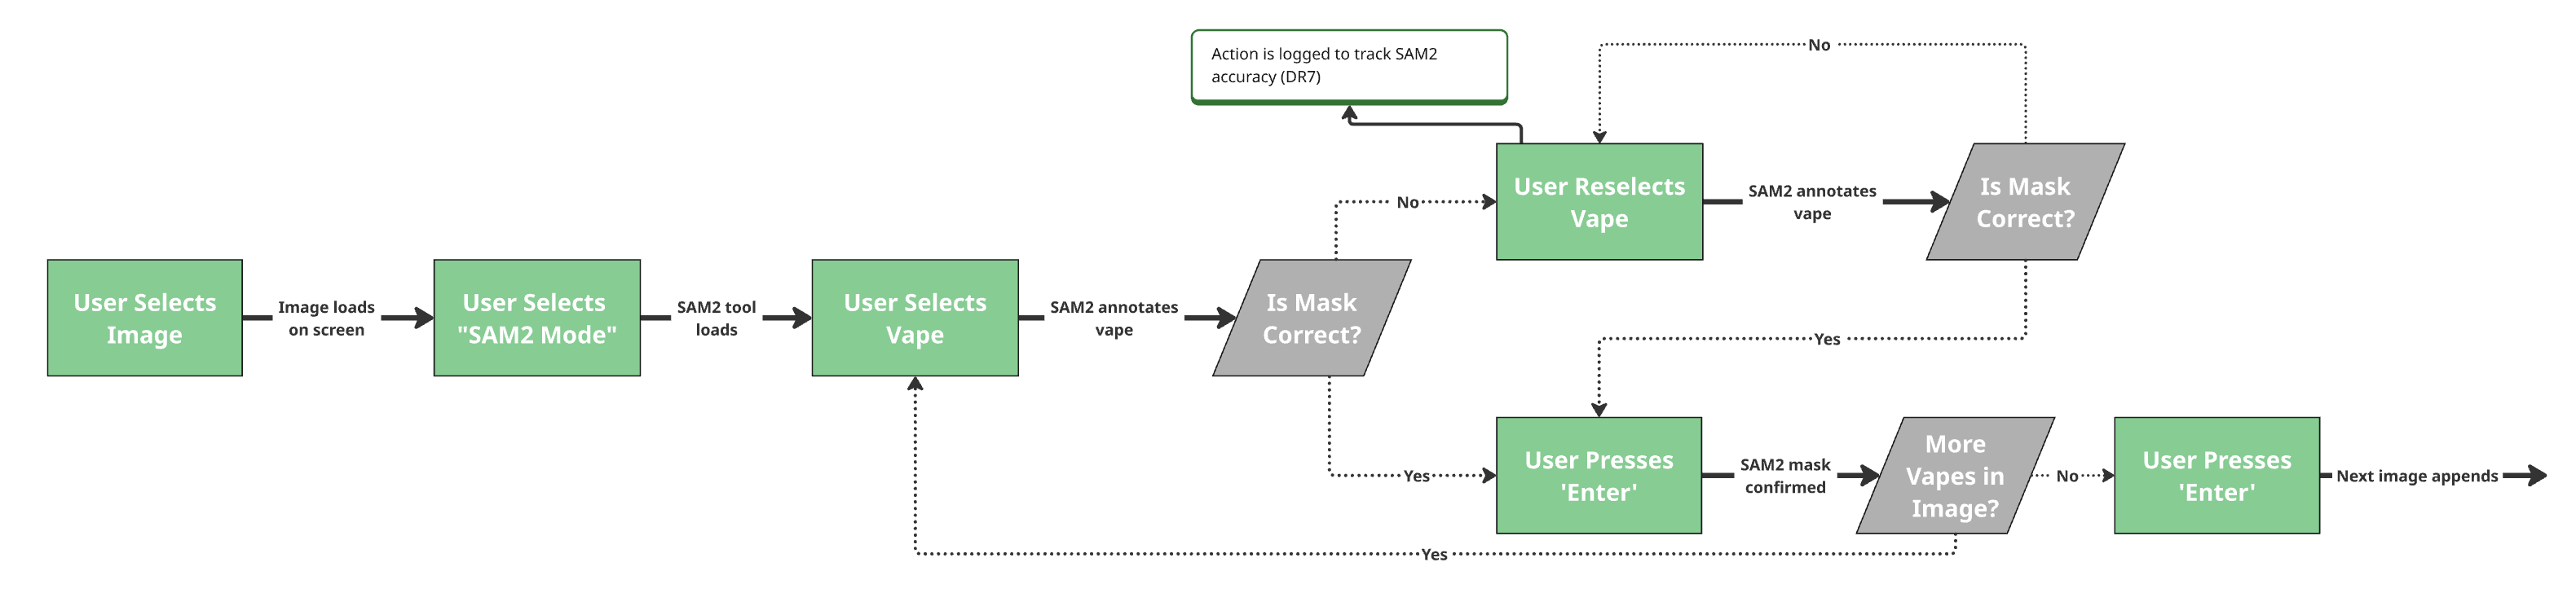
\includegraphics[width=1\linewidth]{SAM2 Flow.png}
    \caption{SAM2 User Interaction Flowchart}
    \label{fig:sam2_interaction_flow}
\end{figure}

\textbf{Validation Benchmark:} To evaluate the annotation workflow, three metrics were defined. First-click accuracy measured the proportion of final accepted annotations that succeeded from the first SAM2 click without requiring a corrective re-click:

\begin{equation}
\label{eq:fca}
FCA = \left(1 - \frac{N_{rc}}{N}\right) \times 100
\end{equation}

\noindent where $N$ is the number of finalised annotations and $N_{rc}$ is the number of those annotations that required at least one corrective re-click.

Because first-click accuracy treats a single correction and multiple corrections equally, interaction efficiency was also defined:

\begin{equation}
\label{eq:interaction_efficiency}
E = \left(\frac{N}{N + R}\right) \times 100
\end{equation}

\noindent where $R$ is the cumulative number of corrective interactions. This metric captures the total mechanical burden of correction rather than only whether a correction occurred.

Finally, mean annotation time was defined as:

\begin{equation}
\label{eq:mean_annotation_time}
t_{avg} = \frac{T_{total}}{N}
\end{equation}

\noindent where $T$ is time in seconds. And time reduction relative to manual annotation was defined as:

\begin{equation}
\label{eq:time_reduction}
TR = \left(1 - \frac{t_{SAM}}{t_{manual}}\right) \times 100
\end{equation}

These time-based metrics were included to evaluate the practical efficiency of the full human-in-the-loop SAM2 annotation workflow.

\vspace{0.5em}
\noindent\textbf{$\rightarrow$ Design requirements addressed:} DCE-DR4.

\subsubsection{Metadata Labelling and VLM Assistance}

Standard object annotation identifies where a target is, but fails to capture the environmental conditions surrounding it. This prevents granular failure-mode analysis (e.g., diagnosing whether a model fails specifically in shadows, high clutter, or on grass). However, forcing users to manually tag these variables across thousands of images introduces severe mechanical fatigue.

To automate this workflow, the DCE integrates a Vision-Language Model (OpenAI GPT-4o-mini) as a metadata assistant \cite{openai_gpt4o_mini_docs}. The VLM strictly classifies image-level variables (surface, lighting, background clutter, object condition, viewpoint, occlusion, and blur) from image inputs \cite{openai_vision_docs}. The system auto-suggests these tags under the hood, allowing the human annotator to simply review, edit, and save them.

The VLM was used only for image-level metadata, not pixel-level annotation. This distinction was important because VLMs are powerful for interpreting contextual features such as \textit{grass background}, \textit{shadow lighting}, or \textit{partial occlusion}.

Two strict engineering rules were applied to this module:
\begin{itemize}
\item \textbf{Token Optimization:} VLM inference is triggered only \textit{after} an image passes the Review Queue, preventing wasted API costs on rejected or uncurated candidates.
\item \textbf{Deterministic Scale:} The ``scale band'' metric is deliberately excluded from the VLM prompt. Instead, it is calculated programmatically by comparing the final SAM2 bounding box area to the total image area, ensuring mathematical accuracy over AI estimation.
\end{itemize}

\begin{figure}[H]
\centering
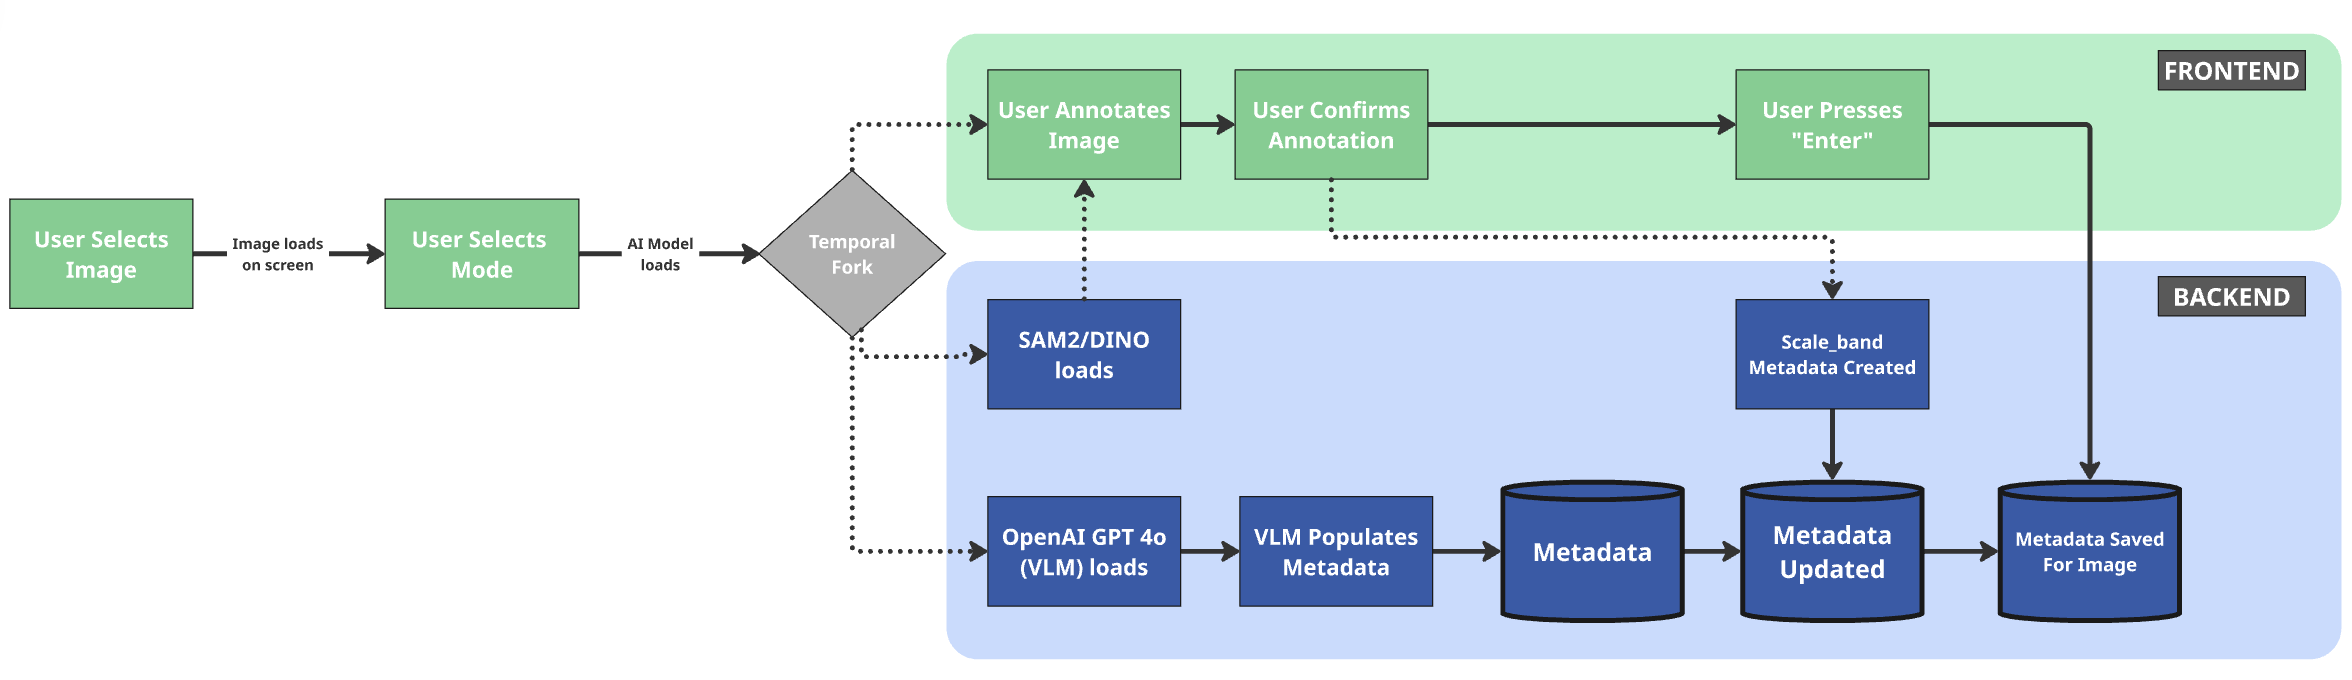
\includegraphics[width=0.8\linewidth]{Metadata_Flow.png}
\caption{Metadata suggestion and review flow within the Dataset Construction Engine.}
\label{fig:metadata_flow}
\end{figure}

\textbf{Validation Benchmark:} This module is validated in two layers. First, VLM API reliability is evaluated by recording the ratio of successful suggestions to API failures. Second, the dataset's overall failure-mode readiness is measured by calculating per-field metadata coverage:

\begin{equation}
\label{eq:metadata_coverage}
M_c = \frac{N_{\text{field}}}{N_{\text{annotated}}} \times 100
\end{equation}

\vspace{0.5em}
\noindent\textbf{$\rightarrow$ Design requirements addressed:} DCE-DR5.

\subsubsection{DCE System Diagram}
The system diagram below summarises the core functionalities of the DCE. The DCE saves the dataset in COCO format and exports it in YOLO format. COCO is used as the source of truth because it preserves polygons, categories, image records, and metadata \cite{lin2014coco}. YOLO is used at export because it provides a lightweight training format suitable for object-detection models and edge-compute deployment \cite{ultralytics_detect_docs}.

\begin{figure}[H]
    \centering
    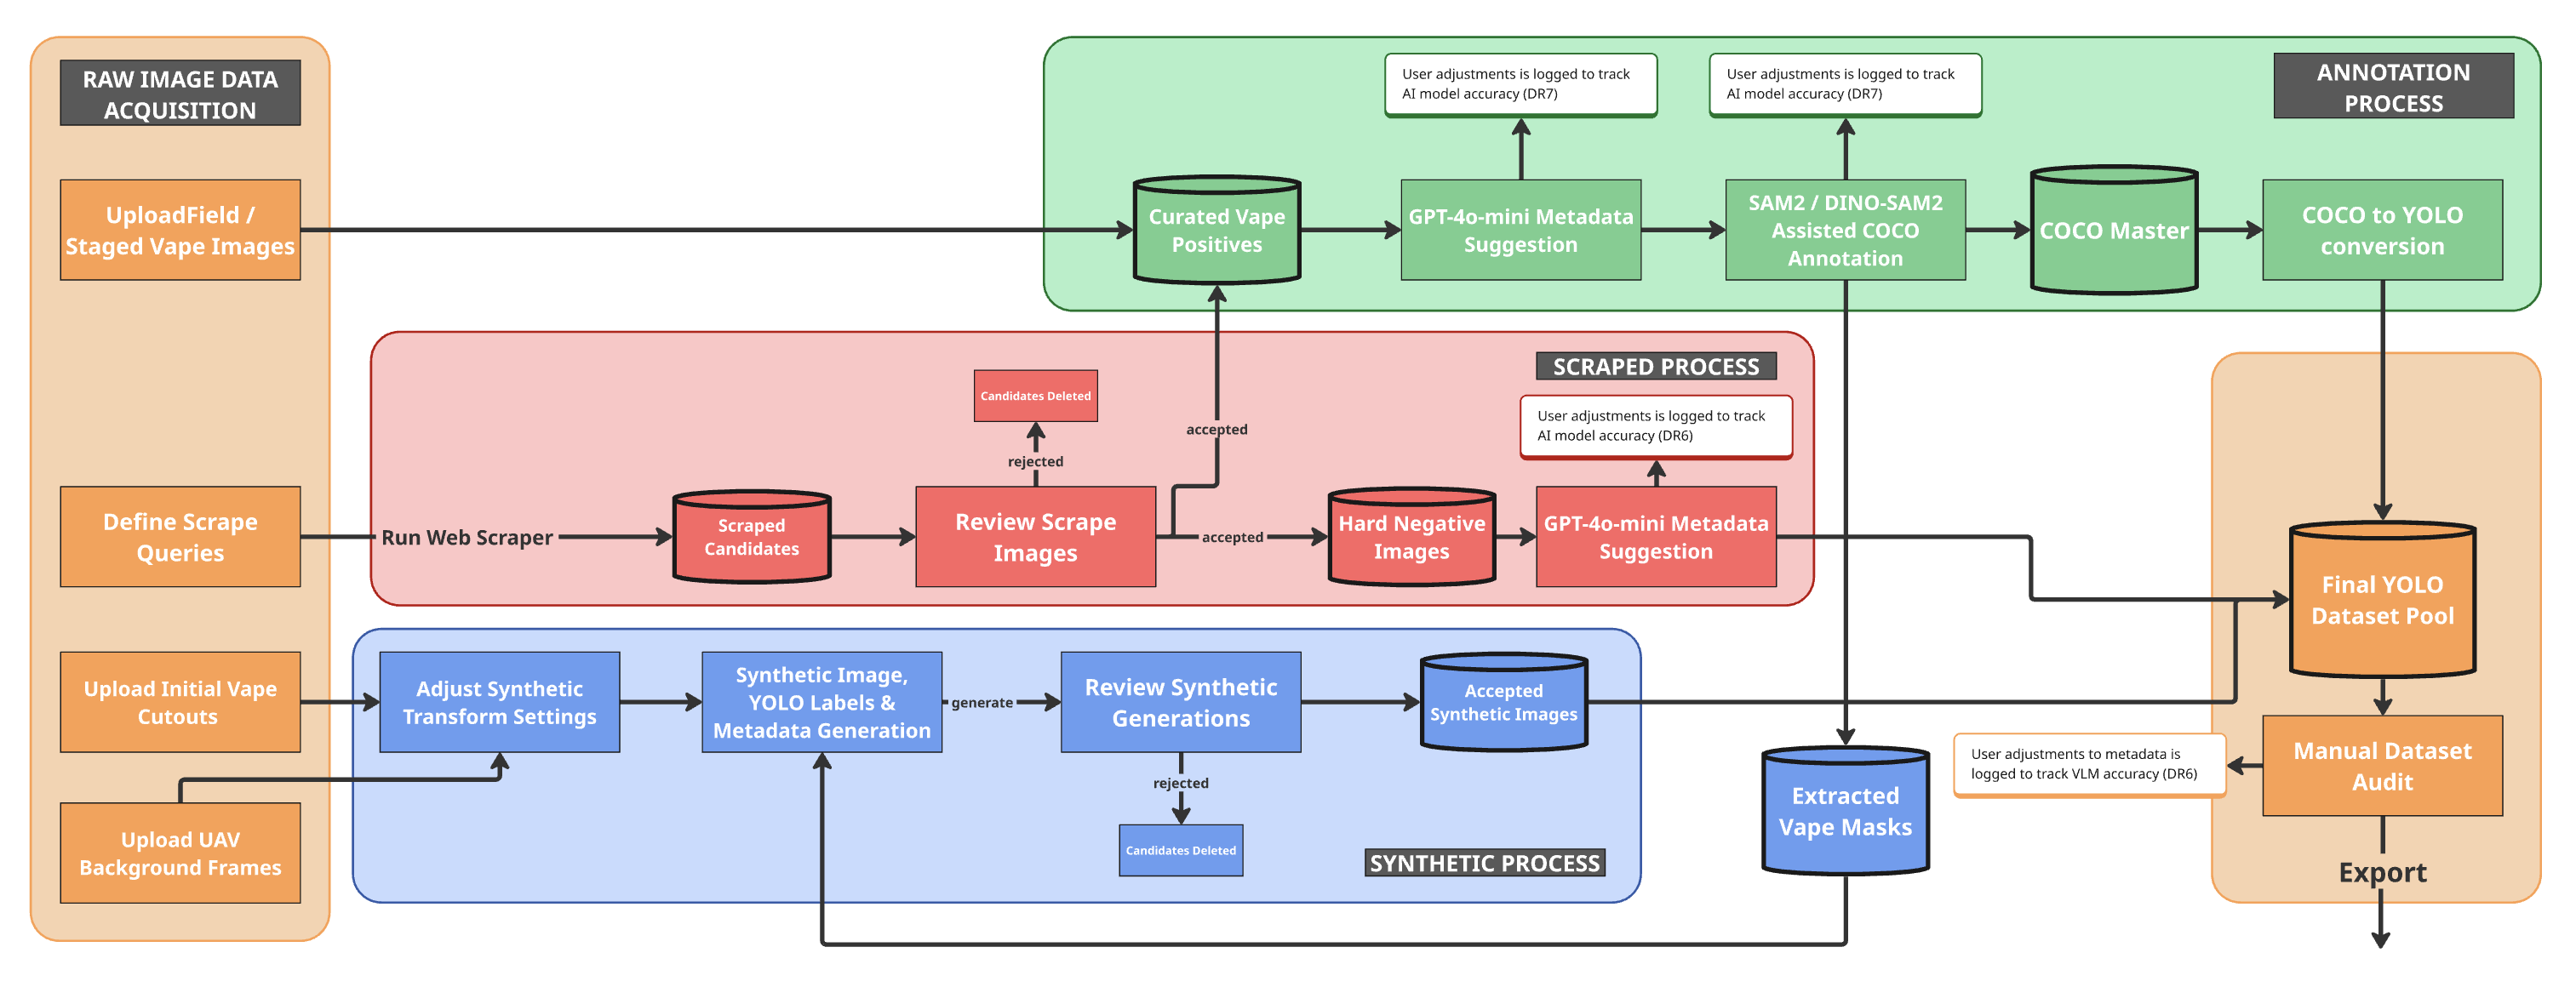
\includegraphics[width=1\linewidth]{DCE System Diagram.png}
    \caption{DCE System Diagram}
    \label{fig:dce_system_diagram}
\end{figure}

\noindent\textbf{$\rightarrow$ Design requirements addressed:} DCE-DR6.

\subsubsection{UI Iterations \& Limitations}

The DCE's UI was iteratively refined throughout development based on repeated use of its core workflows. A limitation is that the DCE was developed and evaluated primarily by the author, rather than tested with a larger group of external users. As a result, the evaluation demonstrates technical functionality and workflow feasibility, but does not fully assess broader usability across different users. This was purposely done as the DCE was developed as a functional research prototype, with future open-source release intended to support wider testing and feedback. System architecture linked in Appendix.


\subsection{UAVape Method}

\textbf{SRQ 2: Machine Perception and Edge Evaluation} How might we train a lightweight edge-vision architecture on a dedicated vape litter dataset to improve the detection-readiness of disposable vapes in urban environments?

\begin{figure}
    \centering
    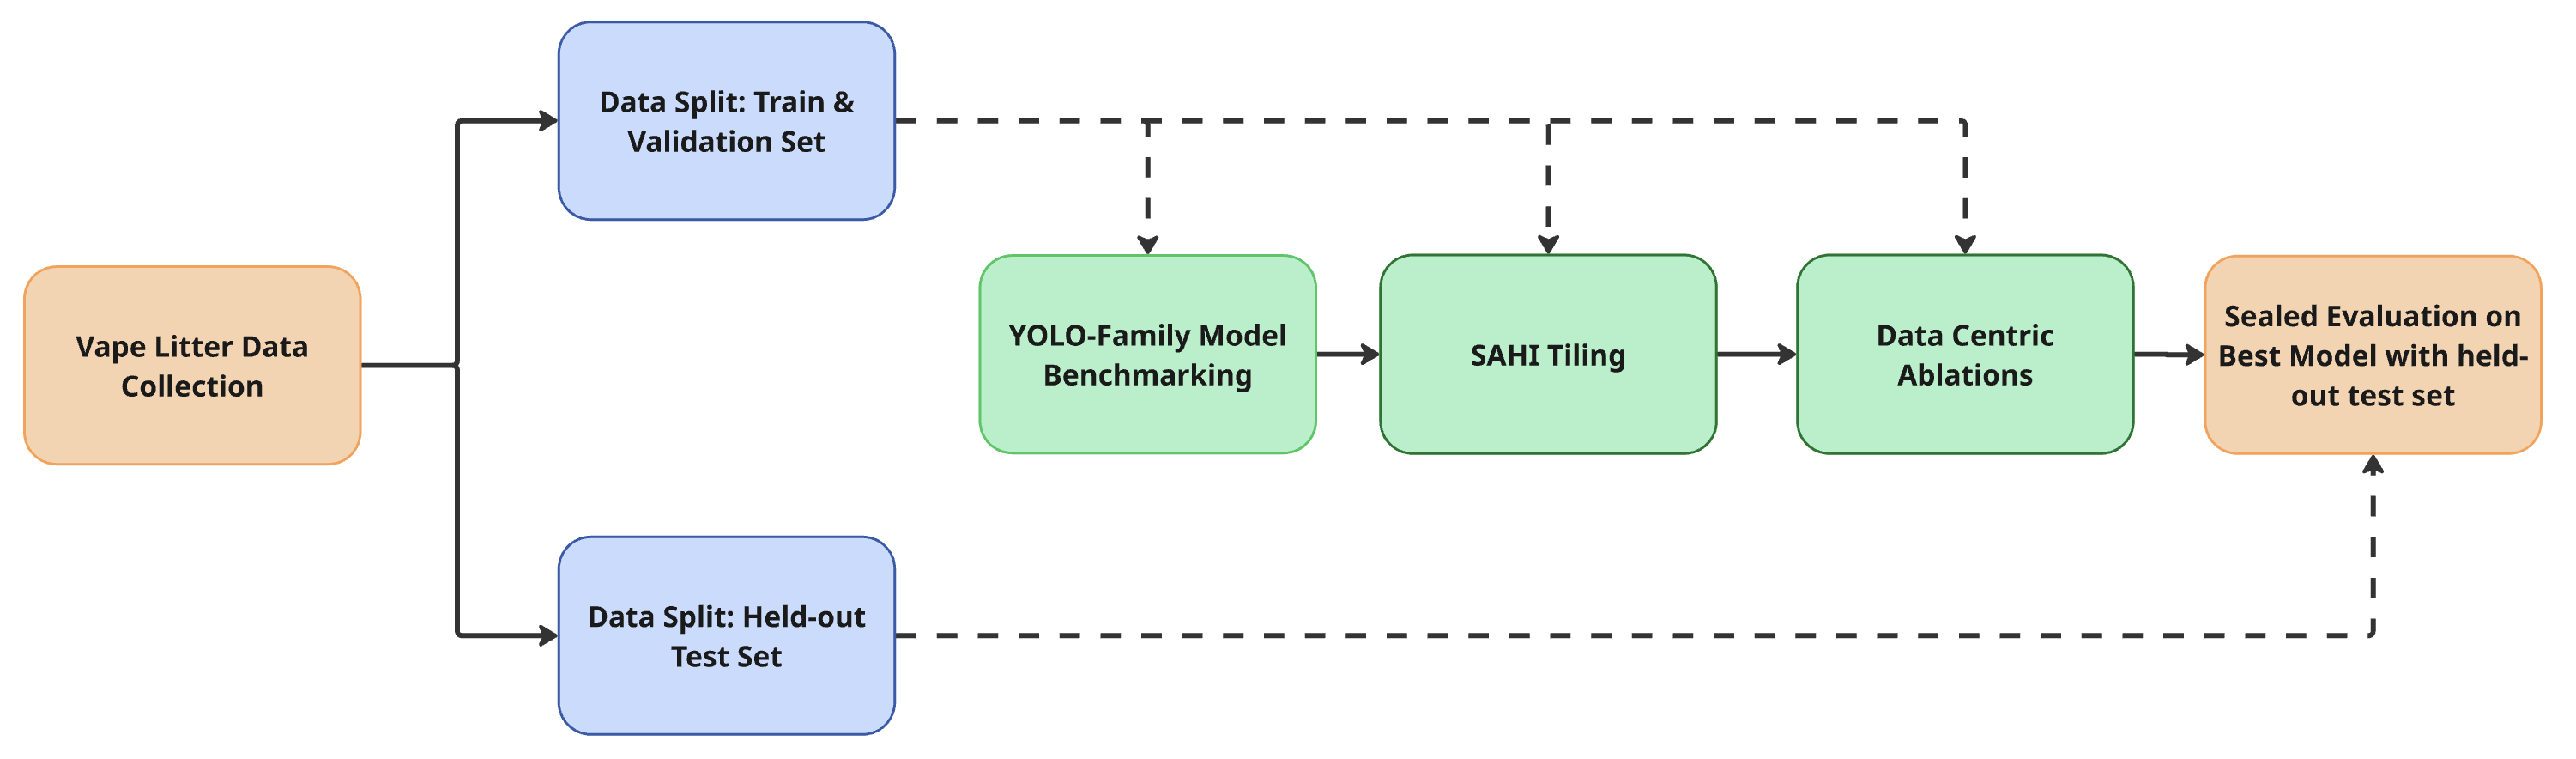
\includegraphics[width=0.5\linewidth]{UAVape Method Overview.png}
    \caption{UAVape Method Overview}
    \label{fig:uavape_method_overview}
\end{figure}

To answer SRQ2, the methodology evaluates how effectively a lightweight edge-vision architecture can detect vapes in urban environments. The experimental design follows a strict four-stage pipeline:
\begin{enumerate}
    \item \textbf{Dataset Assembly:} Constructing a leakage-aware, two-class ground-truth dataset via a structured physical sourcing protocol.
    \item \textbf{Model Benchmarking:} Train the dataset across YOLO architectures, scales, and resolutions.
    \item \textbf{Inference \& Data Ablations:} Testing tiled inference (SAHI) and isolating the impact of the DCE's scraped and synthetic data.
    \item \textbf{Sealed Evaluation:} Testing the final optimal protocol against a sealed, held-out test set.
\end{enumerate}

\subsubsection{Stage 1: Dataset Assembly}
Vapes exhibit massive intra-class variance (brands, colours, degradation) so are highly susceptible to false positives from visual confusers like lighters, pens, and debris.

\begin{figure}[H]
\centering
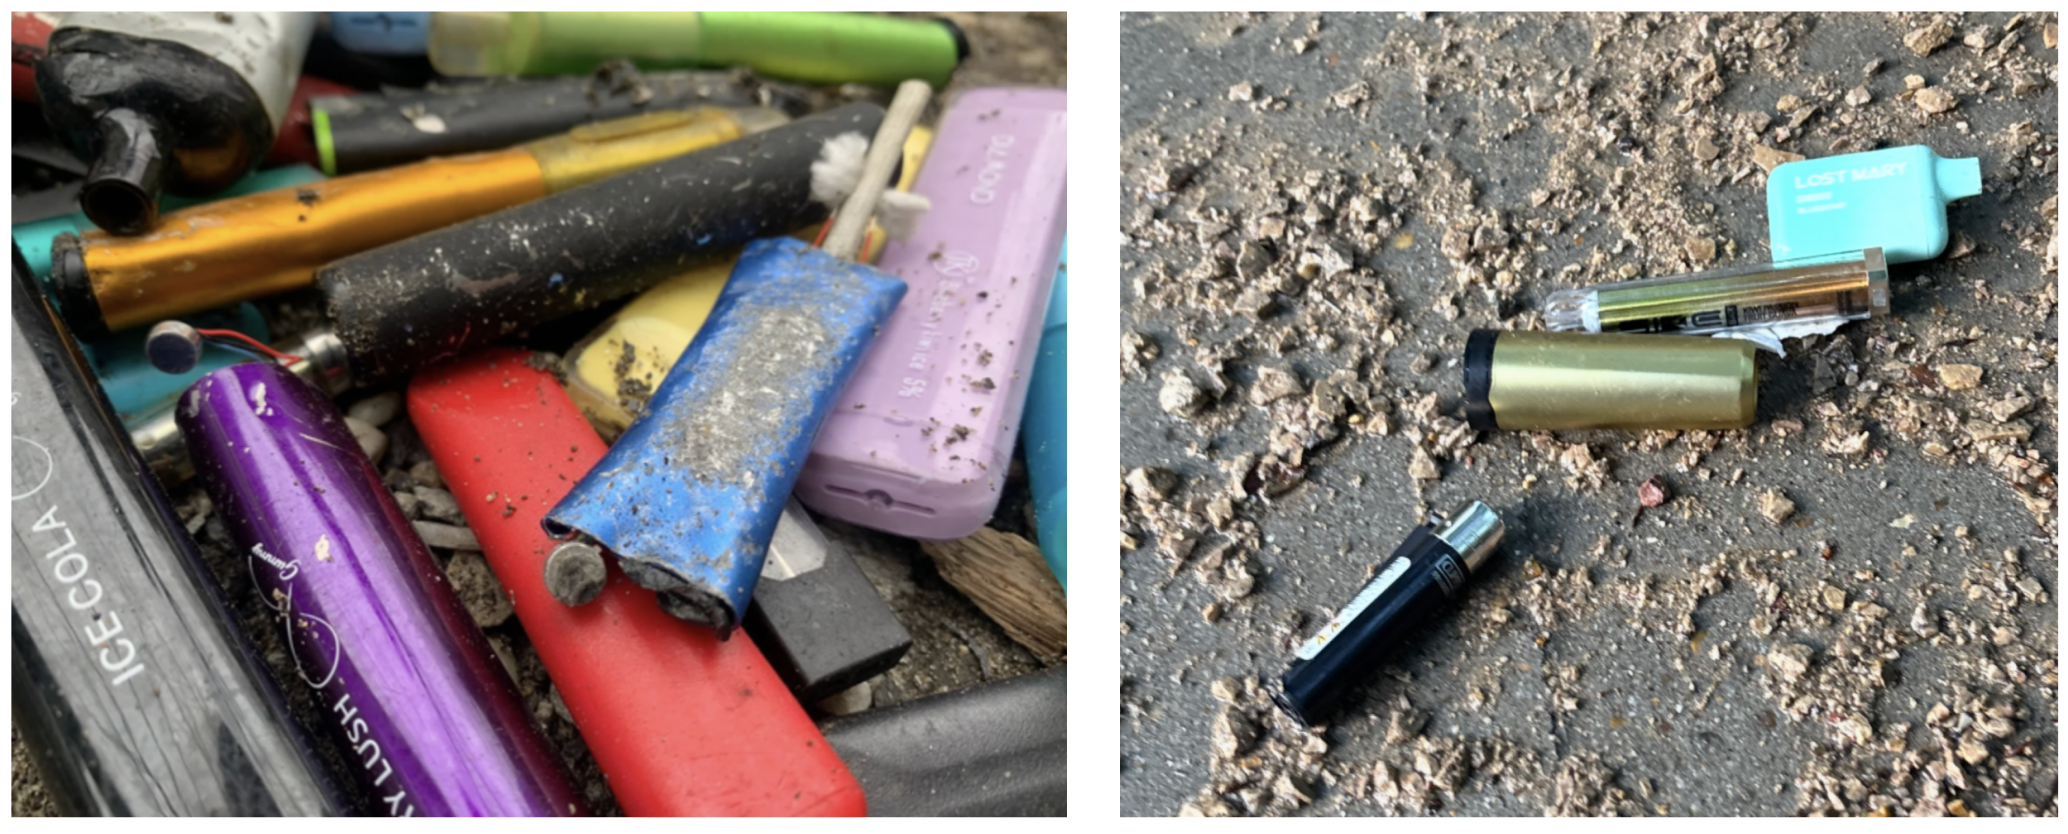
\includegraphics[width=0.7\linewidth]{Screenshot 2026-06-03 at 12.00.40.png}
\caption{Left: Intra-class variance of vape litter. Right: Lighter littered alongside disposable vapes as a visual confuser.}
\label{fig:vape_variance_confuser}
\end{figure}

For this reason, the UAVape dataset was constructed around two classes: (\texttt{0: vape}, \texttt{1: lighter}). Although the ultimate research target is disposable vapes, lighters were explicitly included as an auxiliary (secondary) class to actively penalize vape-lighter false positive confusion. The aim was to explicitly train deep-learning models to distinguish between visually similar disposable vapes and lighters, enabling the model to learn specific features that make a vape unique, rather than learning generic "elongated cylinder" shapes.

For data collection, 25 disposable vapes and 18 lighters were bought. These were selected to cover a range of colours, brands, form factors, and material finishes within project budget limits.

\begin{figure}[H]
    \centering
    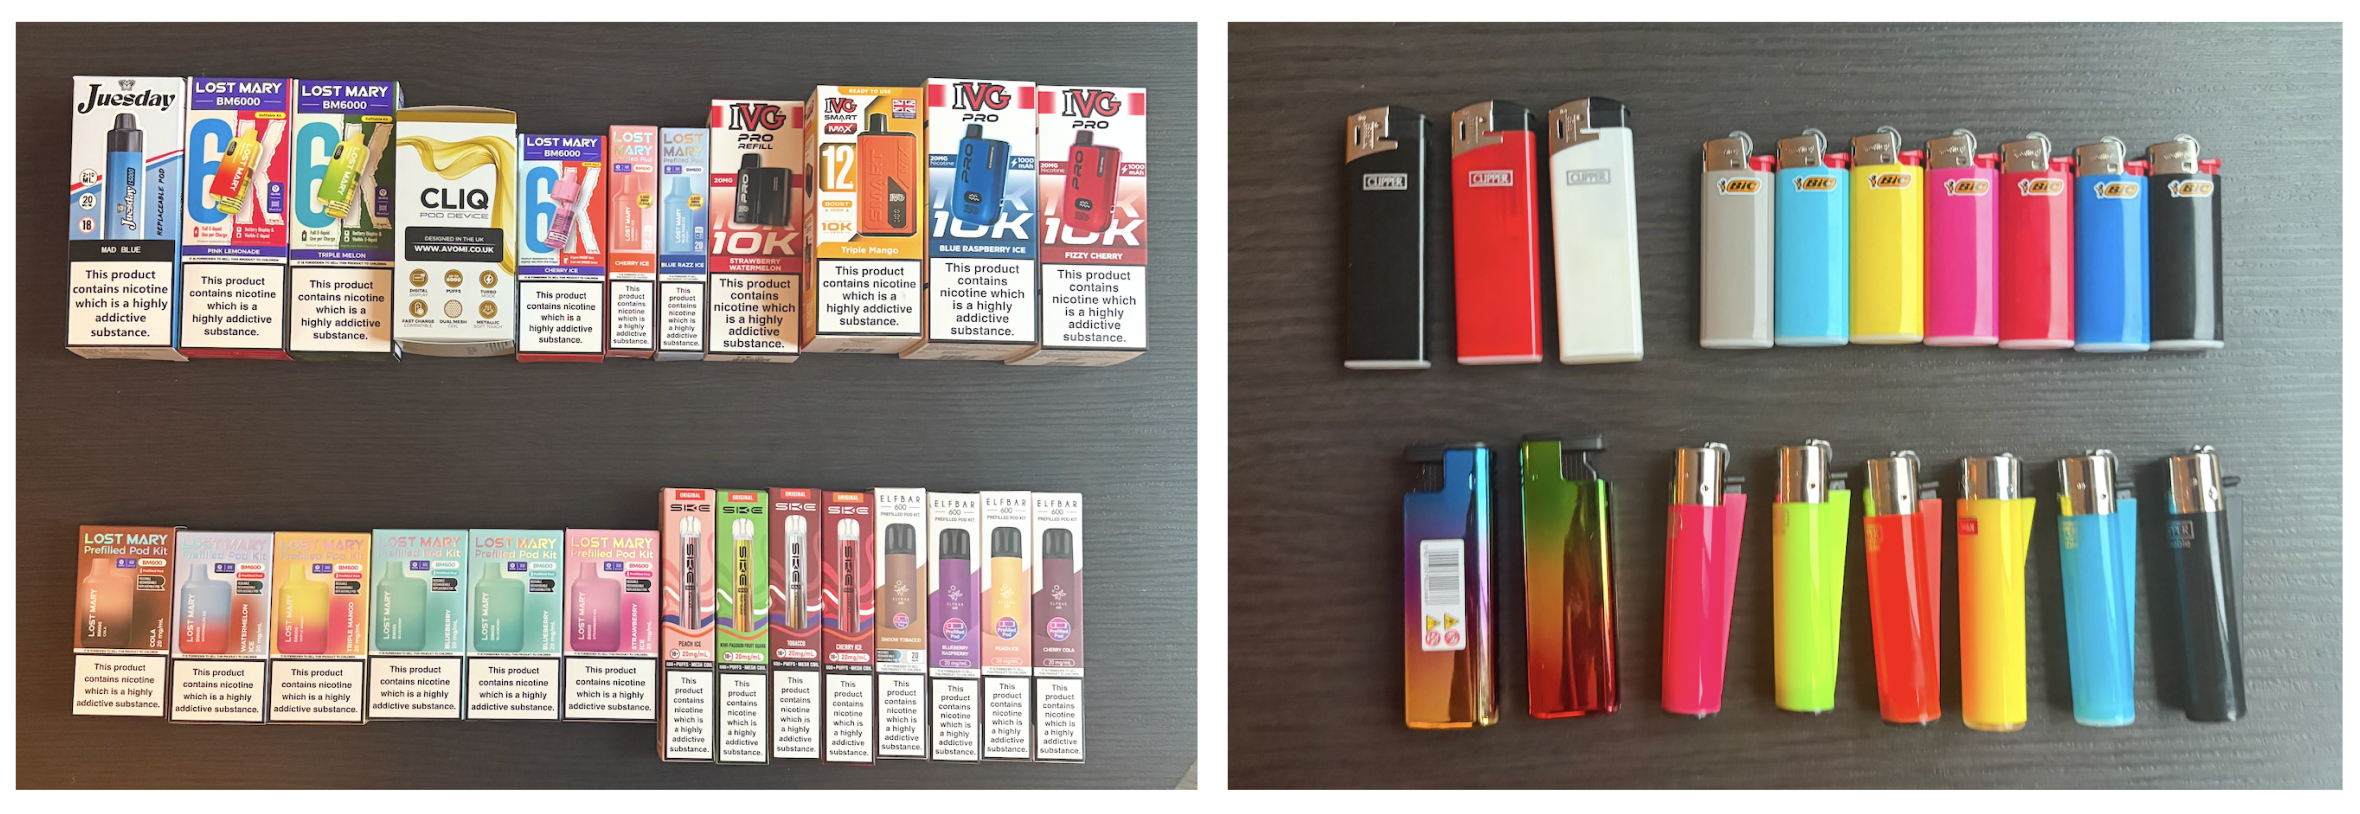
\includegraphics[width=0.7\linewidth]{Screenshot 2026-06-03 at 15.12.37.png}
    \caption{Left: positive vape inventory. Right: auxiliary lighter inventory.}
    \label{fig:uavape_inventory}
\end{figure}

Data collection used three units: station, scene, and frame. A station is one physical ground patch. A scene is one object arrangement at that station. A frame is one captured image, either a photo or a decimated video frame. At each station, three scenes were captured:

\begin{table}[h]
\centering
\begin{tabular}{p{0.18\linewidth} p{0.32\linewidth}}
\hline
Scene & Setup \\
\hline
Scene 1 & One isolated vape \\
Scene 2 & One isolated lighter \\
Scene 3 & Random cluster of  vapes and lighters \\
\hline
\end{tabular}
\end{table}

Because practical constraints prevented live UAV deployment during data collection, an iPhone was used as a controlled low-altitude sensor proxy. The collection protocol was designed to reproduce the core visual challenges of aerial detection: small target scales, oblique viewpoints and environmental clutter. Images were gathered in two separate batches. 

\begin{figure}
    \centering
    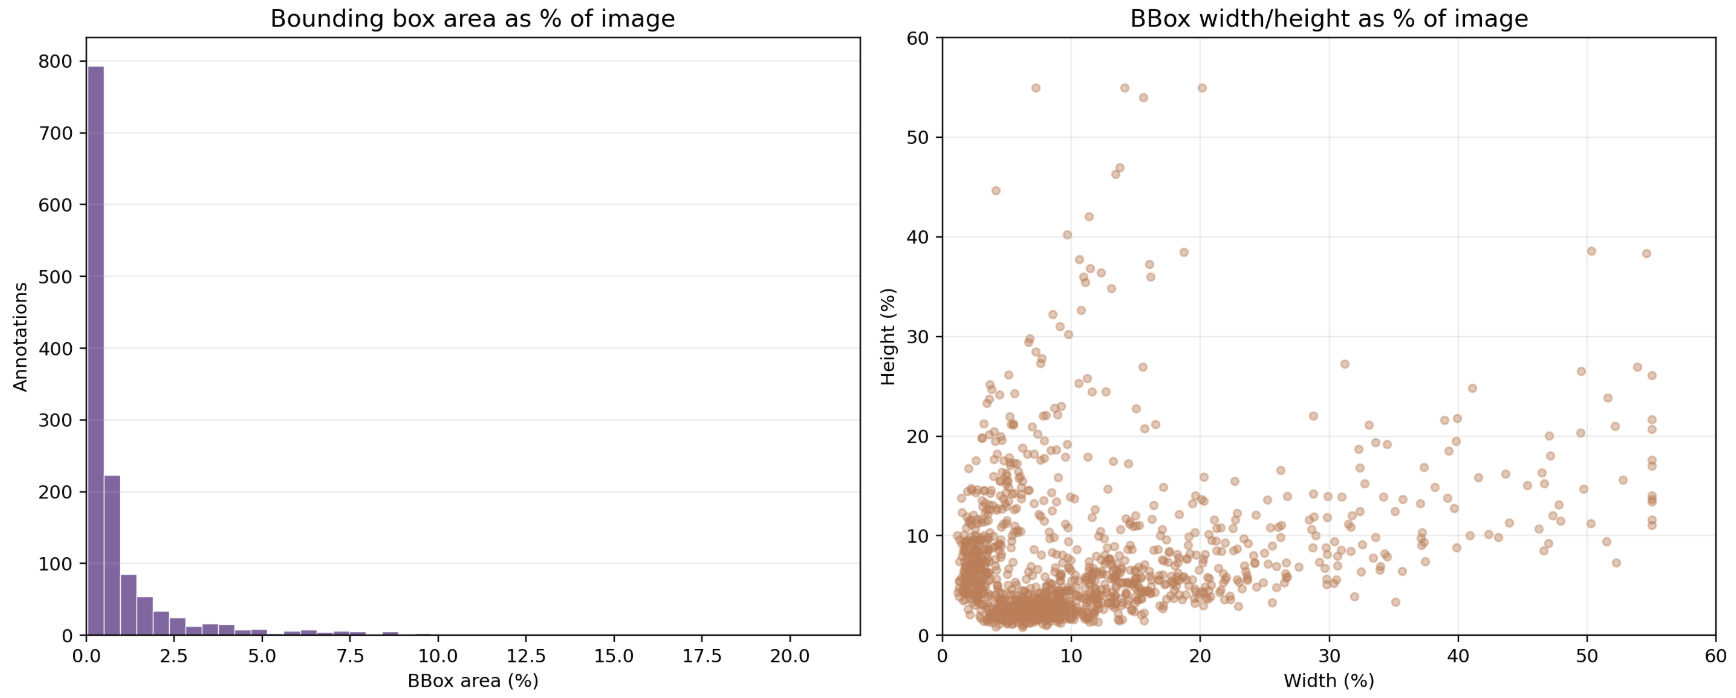
\includegraphics[width=0.8\linewidth]{batch_a_b_bounding_box_sizes.png}
    \caption{Batch A \& B Bounding Box Sizes Examples}
    \label{fig:batch_bbox_examples}
\end{figure}

\begin{table}[H]
\centering
\small
\begin{tabularx}{\textwidth}{X r r r r}
\toprule
\textbf{Source pool} & \textbf{Images} & \textbf{Vape boxes} & \textbf{Lighter boxes} & \textbf{Total boxes} \\
\midrule
Batch A & 641 & 670 & 275 & 945 \\
Batch B & 563 & 658 & 437 & 1095 \\
\textbf{Combined final real dataset} & \textbf{1204} & \textbf{1328} & \textbf{712} & \textbf{2040} \\
\bottomrule
\end{tabularx}
\caption{Final real-image composition of the UAVape detector dataset.}
\label{tab:uavape_final_dataset_composition_method}
\end{table}

The images were then uploaded to the DCE, audited and annotated. Results of this process is outlined in Section 6.

\subsubsection{Leakage-Aware Data Split}

Before training the detector, the labelled images were divided into train, validation and test sets. The training set is used to fit the model weights. The validation set is used during development to compare model settings and select the strongest protocol. The test set is held back until the end to estimate how well the final selected detector generalises to unseen data.

This split was constructed around scene-level independence. The data collection process deliberately captured repeated views of related objects, surfaces and placements to increase scale and viewpoint variation. These related frames are useful for training, but they should not be scattered across train, validation and test sets. If repeated views of the same scene appear in both training and testing, the evaluation may overfit: rewarding the recognition of familiar backgrounds rather than generalisation to new capture contexts.

For this reason, related capture groups were kept together where possible. The train and validation sets used Batch A together with a subset of Batch B, while the test set was drawn only from the remaining Batch B groups. This preserved a held-out real-image test set while reducing the risk that near-duplicate views of the same scene appeared across development and final evaluation splits.

\begin{table}[H]
\centering
\small
\begin{tabularx}{\textwidth}{l r r r r r r}
\toprule
\textbf{Split} & \textbf{Images} & \textbf{Vape boxes} & \textbf{Lighter boxes} & \textbf{Old images} & \textbf{New images} & \textbf{Groups} \\
\midrule
Train & 837 & 870 & 447 & 525 & 312 & 87 \\
Validation & 183 & 203 & 100 & 116 & 67 & 10 \\
Test & 184 & 255 & 165 & 0 & 184 & 19 \\
\bottomrule
\end{tabularx}
\caption{Leakage-aware train, validation and test split used for UAVape V4.}
\label{tab:uavape_results_split}
\end{table}

The resulting split corresponds to approximately 69.5\% training, 15.2\% validation and 15.3\% testing by image count. This is close to the common 70/15/15 split used in supervised machine-learning workflows, while prioritising the prevention of scene-level data leakage over exact ratio matching.

\subsubsection{Stage 2: The Unified Model Benchmark}
A unified benchmark was conducted across three primary variables: \textbf{Architecture Family}, \textbf{Model Scale}, and \textbf{Input Resolution (\texttt{imgsz})}.

To determine the most viable edge-compute detector, the benchmark tested YOLOv8 (the literature standard), YOLO11 (modern baseline), and YOLO26 (the newest Ultralytics candidate) \cite{ultralytics_yolov8_docs,ultralytics_yolo11_docs,ultralytics_platform_docs}. UAV deployment feasibility was considered so testing centered on Small and Nano scales, with a Medium scale included strictly as a capacity check. Finally, input resolutions were scaled from 640px to 1280px to evaluate the trade-off between computational cost and small-object spatial preservation. 

\begin{table}[H]
\centering
\small
\renewcommand{\arraystretch}{1.2}
\begin{tabularx}{\textwidth}{@{} p{0.25\textwidth} X @{}}
\toprule
\textbf{Benchmark Variable} & \textbf{Tested Parameters} \\
\midrule
\textbf{Model Family} & YOLOv8, YOLO11, YOLO26 \\
\textbf{Model Scale} & Nano (n), Small (s), Medium (m) \\
\textbf{Input Resolution} & 640 (Baseline), 960 (Intermediate), 1280 (High-Detail) \\
\textbf{Training Protocol} & Ultralytics 8.4.62, RunPod H100, 100 Epochs, Cosine LR, Seed 42 \\
\bottomrule
\end{tabularx}
\caption{The experimental matrix for the unified detector-selection benchmark.}
\label{tab:uavape_benchmark_matrix}
\end{table}

\subsubsection{Stage 3: Inference Protocol \& Data-Centric Ablations}
After the baseline unified benchmark was completed, two advanced validation branches were executed before any held-out testing occurred:

\begin{itemize}
    \item \textbf{Tiled Inference (SAHI):} Because small objects are often degraded during the YOLO downsampling phase, Slicing Aided Hyper Inference (SAHI) was investigated as a validation-only inference strategy \cite{akyon2022sahi}. The image was sliced into 1280-pixel tiles with 20\% overlap so that small objects occupied a larger proportion of each inference crop, while the underlying YOLO weights and training procedure remained unchanged.    
    \item \textbf{Data-Centric Ablation (Dose-Response):} To investigate if diverse data sources in this domain could improve the model, a dose-response data ablation study was conducted. 
\end{itemize}

Enabled by the DCE, two external vape-focused data sources were constructed: 355 scraped vape images and 355 synthetic vape composites. Scraped and synthetic additions were introduced at approximately 25\%, 50\% and 100\% of the available external source pool. A final combined-source condition then added the full scraped and synthetic pools together. This structure allowed the experiment to measure not only whether DCE-generated data improved performance, but also whether performance changed monotonically as additional scraped or synthetic images were added.

\begin{table}[H]
\centering
\small
\renewcommand{\arraystretch}{1.2}
\begin{tabularx}{\textwidth}{@{} l X @{}}
\toprule
\textbf{Ablation Pipeline} & \textbf{Tested Doses (Images Added to Baseline)} \\
\midrule
\textbf{Real-Only (Baseline)} & 0 (fixed real-world training set) \\
\textbf{Scraped-Only Addition} & +88, +177, +355 scraped images \\
\textbf{Synthetic-Only Addition} & +88, +177, +355 synthetic composites \\
\textbf{Combined Addition} & +355 scraped images +355 synthetic composites \\
\bottomrule
\end{tabularx}
\caption{Dose-response data ablation matrix used to isolate the impact of DCE-enabled external data sources under a fixed YOLO26s@1280 detector protocol.}
\label{tab:data_ablation_matrix}
\end{table}

The combined condition was evaluated at the full-source setting rather than at every intermediate dose, because the intermediate ablations were intended to isolate the dose-response behaviour of each source independently. The combined run was then used to test whether the two complete source pools provided complementary information when used together.

\subsubsection{Stage 4: Metric Hierarchy and the Sealed Test Set}

Because vapes are hazardous environmental objects, the operational priority is minimizing environmental false negatives (missed vapes). The reporting hierarchy follows standard AP/mAP object-detection reporting conventions \cite{lin2014coco,ultralytics_metrics_docs}, and was therefore defined as follows:

\begin{table}[H]
\centering
\small
\renewcommand{\arraystretch}{1.2}
\begin{tabularx}{\textwidth}{@{} r p{0.28\textwidth} X @{}}
\toprule
\textbf{Priority} & \textbf{Metric} & \textbf{Role in Evaluation} \\
\midrule
1 & Vape AP50 & Headline metric for UAV/litter literature comparability. \\
2 & Vape AP50--95 & Secondary stricter localisation-quality metric. \\
3 & Vape Precision / Recall & Operational behaviour (false alarms vs. missed vapes). \\
4 & Lighter Metrics & Auxiliary diagnostic for confuser-class boundary learning. \\
5 & Aggregate Two-Class mAP & General context only (averages primary and auxiliary classes). \\
\bottomrule
\end{tabularx}
\caption{Metric hierarchy prioritizing target-class localization over generalized multi-class metrics.}
\label{tab:uavape_metric_hierarchy}
\end{table}

Crucially, the held-out Test set was entirely sealed during the execution of Stages 1 through 3. It was not used to select epochs, tune hyperparameters, determine input sizes, evaluate tiling settings, or dictate data recipes. After the final protocol was identified via the validation set, the \texttt{best.pt} checkpoint was evaluated exactly once on the held-out test split to provide an uncompromised estimate of held-out static-image generalisation.

\vspace{0.5em}
\noindent\textbf{$\rightarrow$ Design requirements addressed:} EVAL-DR1, EVAL-DR2, EVAL-DR3, EVAL-DR4.
\subsection{Cleaner Workflow Prototype Method}

\textbf{SRQ 3: Cleaner Workflow UI.} How can raw spatial bounding-box detections be translated into an interactive, evidence-backed workflow interface to improve visibility, prioritisation and hazard verification for frontline cleanup operations?

Building on the cleaner investigation in Section 3, this workstream developed a workflow prototype for translating vape detections into cleanup tasks. The aim was not to test live UAV deployment or real-time geolocation. Instead, the prototype tested whether detection outputs could be represented in a way that was understandable and useful to frontline stakeholders.

The prototype was designed around one workflow: a detected vape becomes an evidence-backed cleanup task. This workflow contains both supervisor-facing screens and cleaner-facing screens. Supervisor-facing screens support review, prioritisation and assignment. Cleaner-facing screens support field collection, evidence checking and status reporting.

\subsubsection{Workflow Outline}

The prototype was structured around six core workflow elements: evidence, location, confidence, hazard identity, assignment and outcome reporting. These elements were selected because a bounding box alone does not tell a cleaner what to collect, where to find it, why it matters or whether it has been removed.

\begin{table}[H]
\centering
\small
\begin{tabularx}{\textwidth}{p{0.28\textwidth} X}
\toprule
\textbf{Workflow element} & \textbf{Purpose} \\
\midrule
Image evidence crop & Allows the user to inspect the detected object rather than relying only on a model output. \\
Map point or spatial marker & Gives the user location context for search and collection. \\
Confidence score & Shows model certainty and supports human review. \\
Hazard label & Preserves disposable vapes as hazardous micro-WEEE rather than generic litter. \\
Task priority and assignment & Allows detections to be converted into cleanup jobs. \\
Task status and proof of cleanup & Records whether the item was collected, not found or requires review. \\
\bottomrule
\end{tabularx}
\caption{Cleaner workflow mapping from detection output to task information.}
\label{tab:cleaner_method_detection_task_mapping}
\end{table}

Initial wireframes were created to define the workflow logic before visual design decisions were made. The wireframes focused on how a detection becomes a task, how it is reviewed and assigned, and how the field outcome is recorded.

\begin{figure}[H]
    \centering
    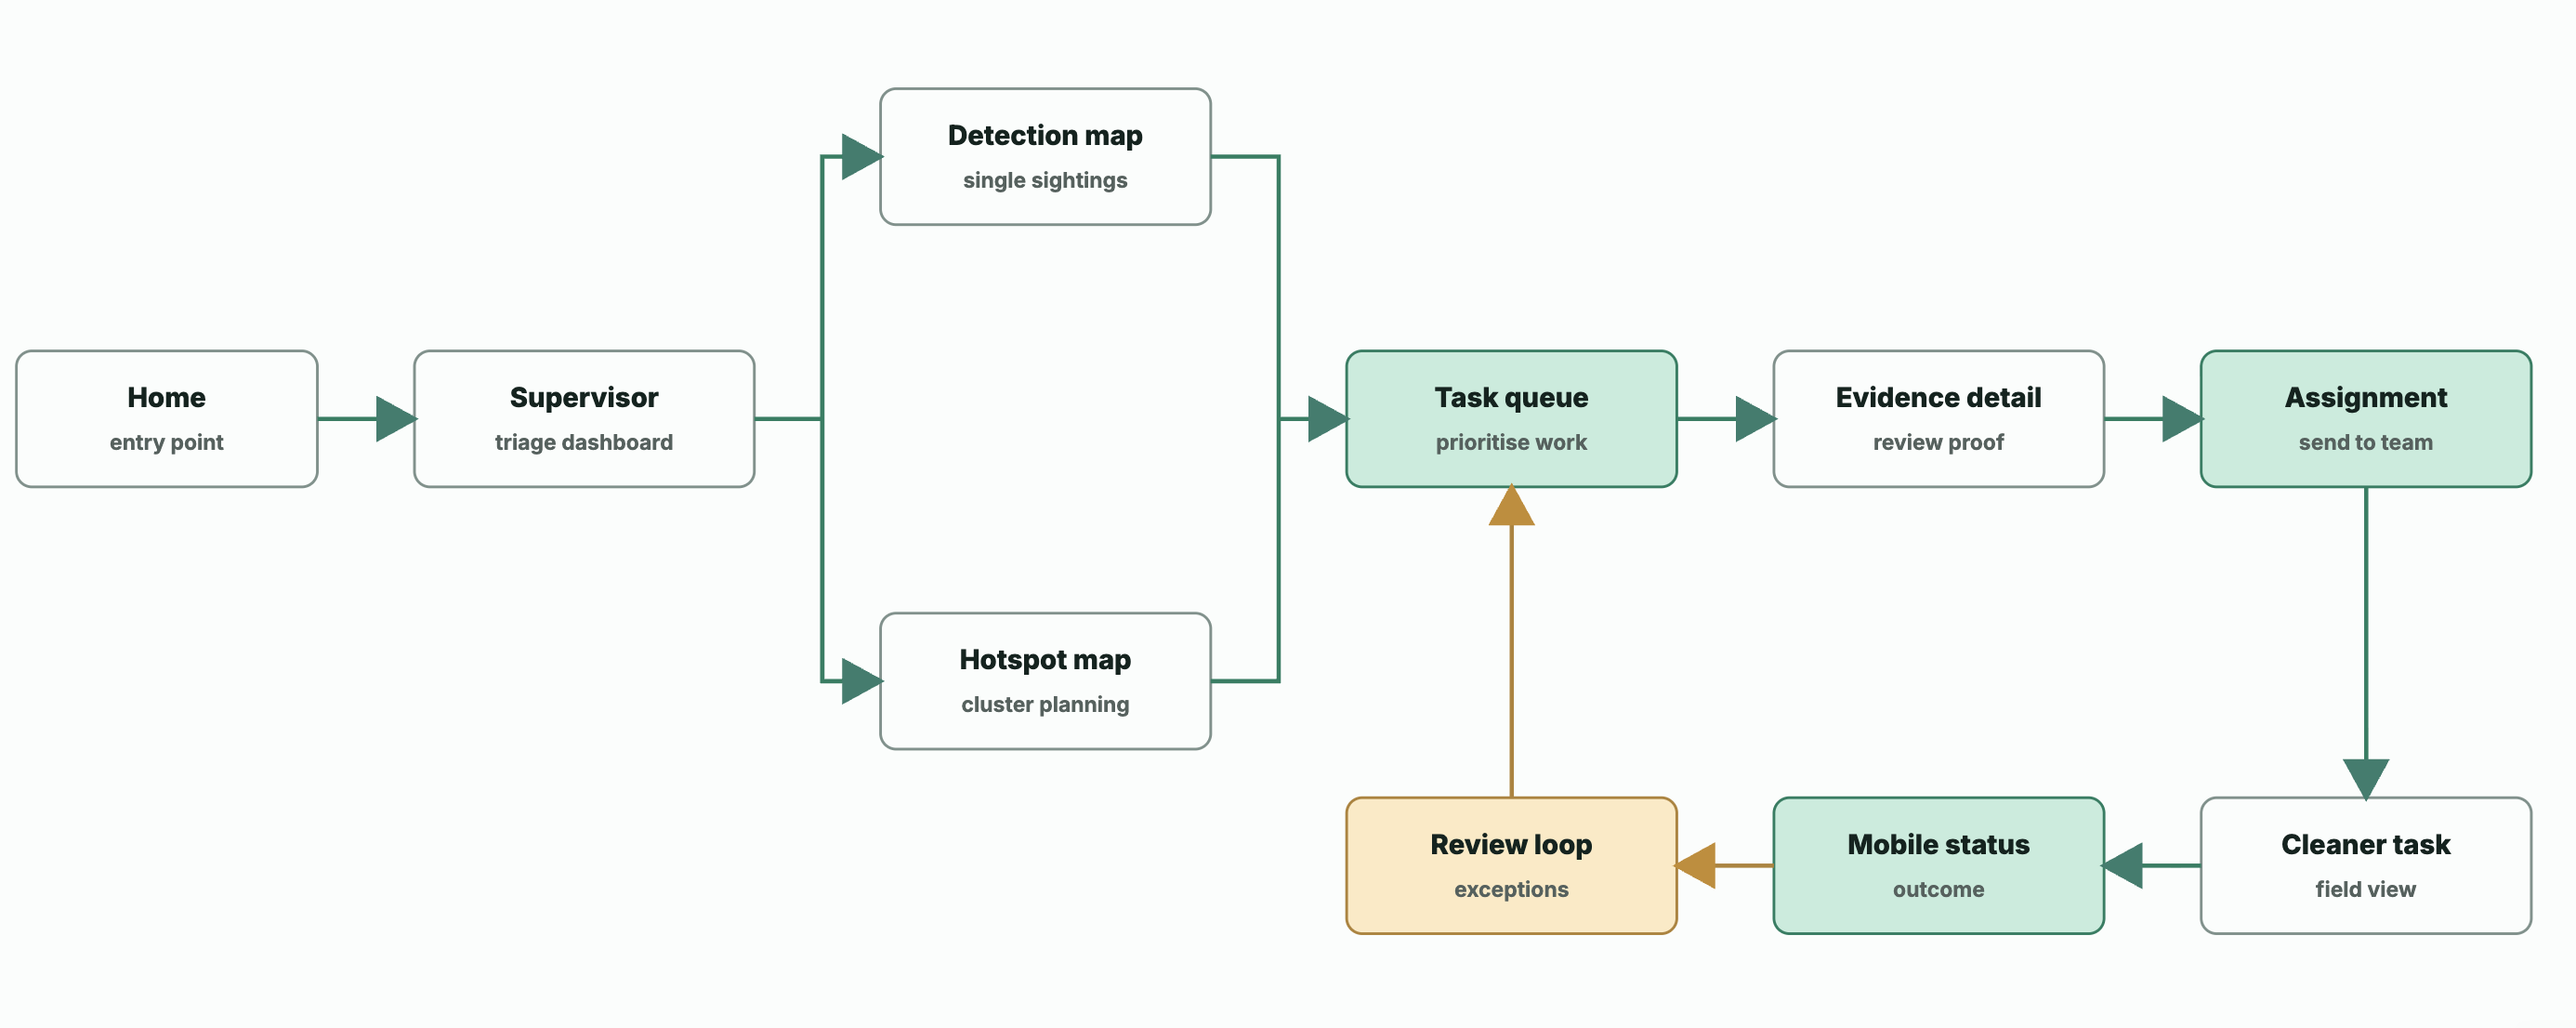
\includegraphics[width=0.9\linewidth]{Wireframes.png}
    \caption{Wireframe planning for the UAVape Cleanup Planner workflow.}
    \label{fig:cleaner_method_wireframes}
\end{figure}

\subsubsection{Low-Fidelity Prototyping}

The wireframes were then developed into low-fidelity prototypes to explore the composition of each screen and the basic user interaction flow.

\begin{figure}[H]
    \centering
    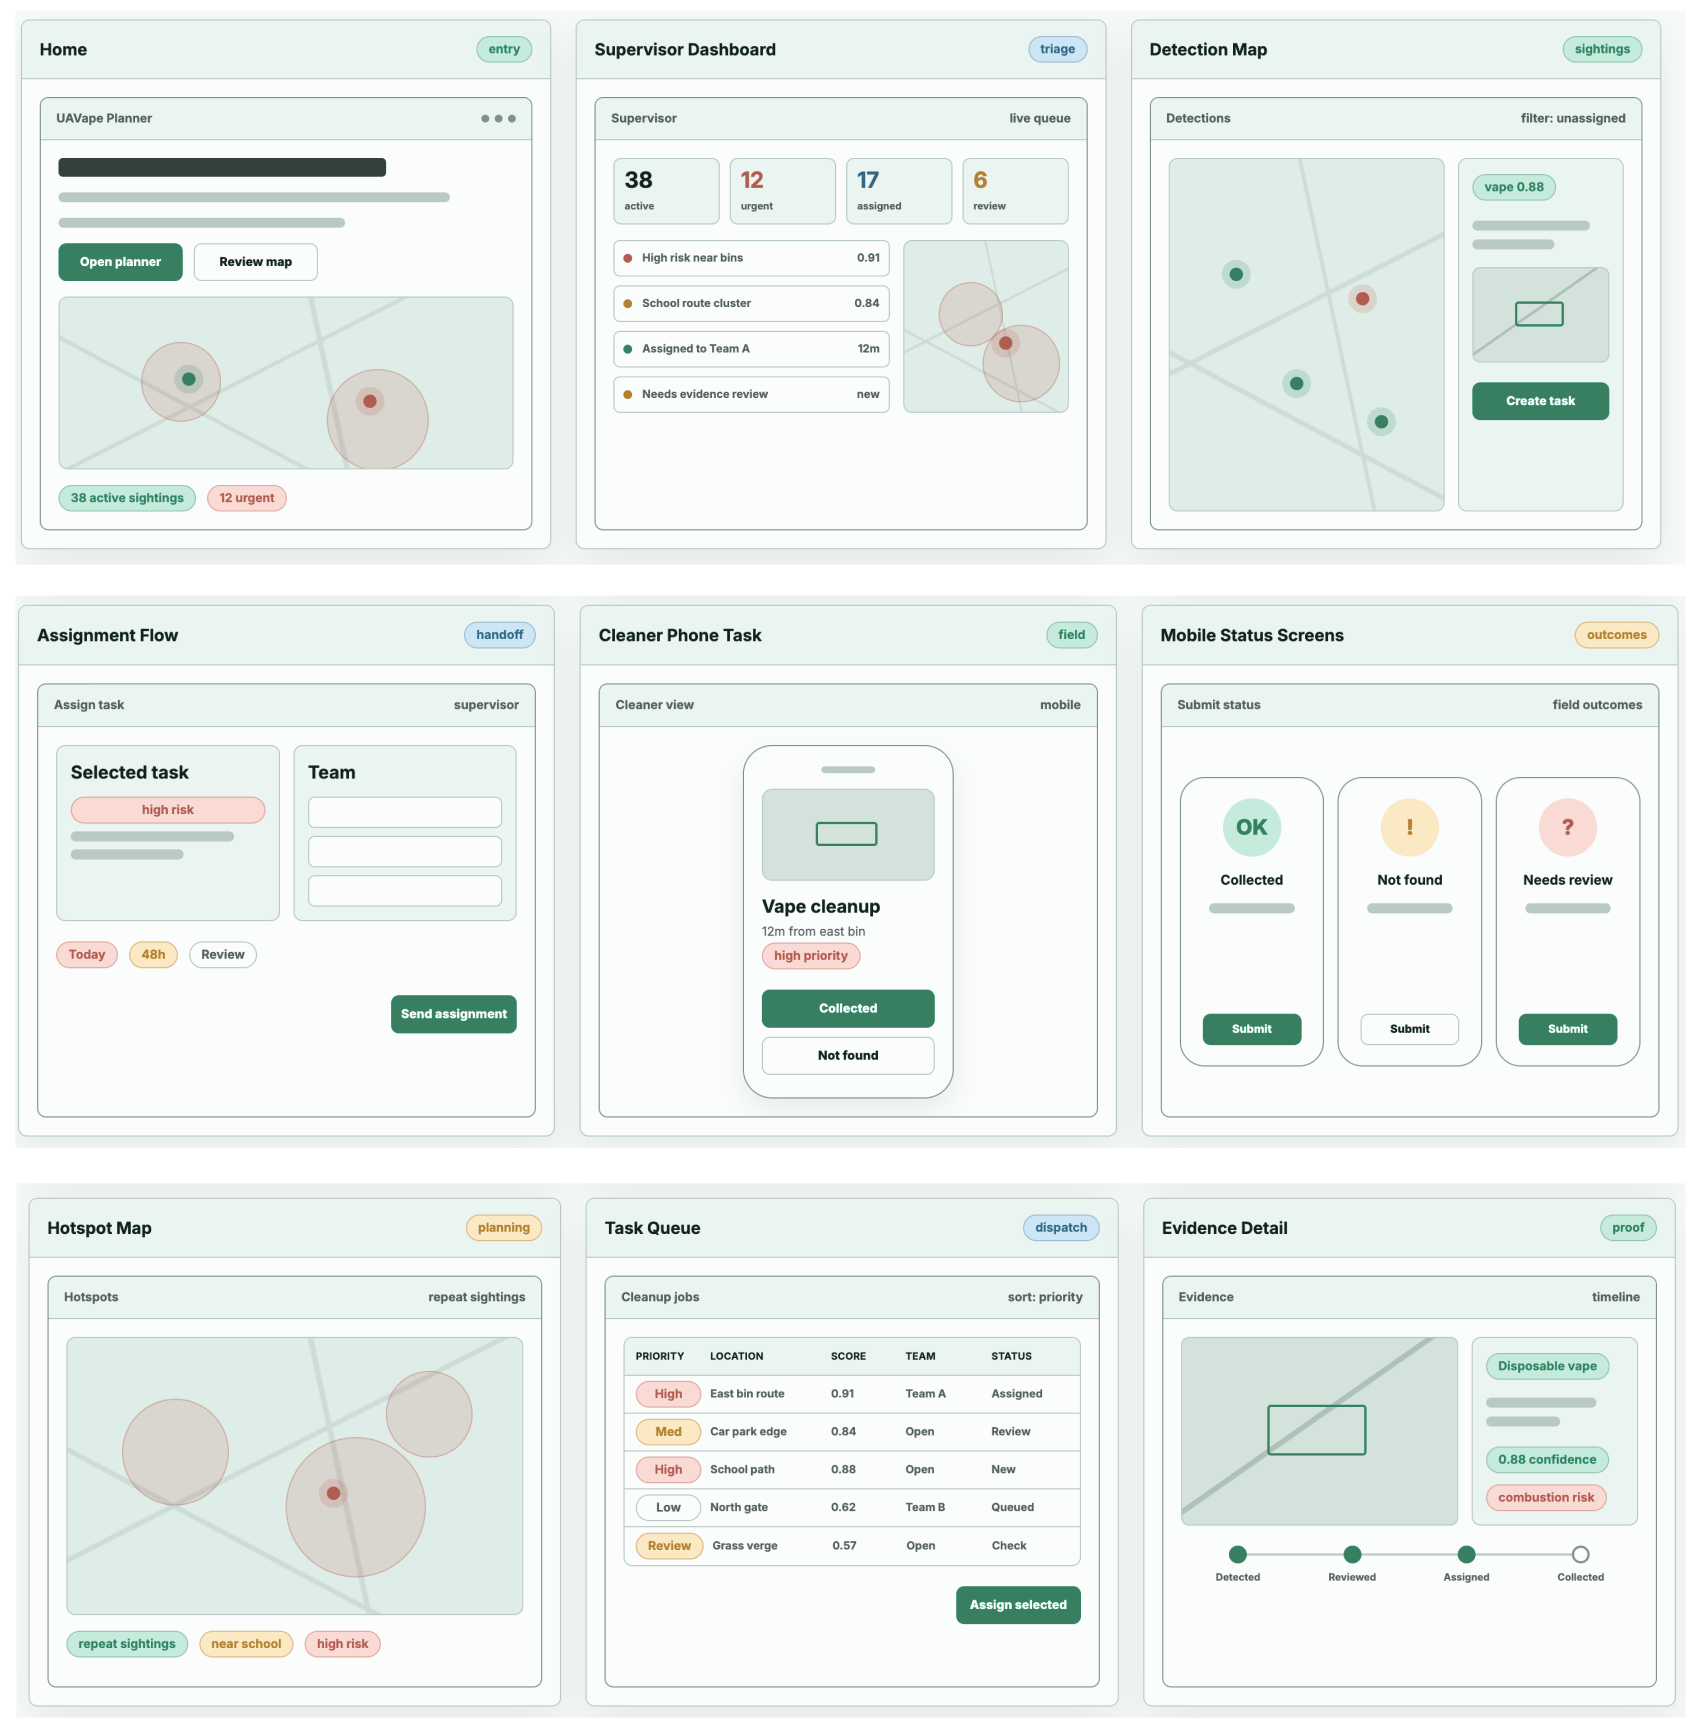
\includegraphics[width=0.9\linewidth]{LOFI.png}
    \caption{Low-fidelity prototype screens for the UAVape Cleanup Planner.}
    \label{fig:cleaner_method_lofi}
\end{figure}

\subsubsection{Stakeholder Walkthrough and Questionnaire}

The prototype was evaluated through a single structured walkthrough with 11 frontline stakeholders, consisting of seven community volunteers and four Veolia operatives. Participants reviewed the full prototype workflow, including both supervisor-facing and cleaner-facing screens. The evaluation did not test live UAV detections, GPS accuracy or real municipal deployment. It tested perceived workflow clarity, usefulness and feasibility.

After the walkthrough, participants completed a short questionnaire. The questions were organised around workflow functions rather than separate participant job roles: evidence and location clarity, confidence and hazard communication, prioritisation, assignment, field usability, status reporting, overall clarity and practical friction.

\begin{table}[H]
\centering
\small
\begin{tabularx}{\textwidth}{p{0.09\textwidth} X p{0.24\textwidth}}
\toprule
\textbf{Q} & \textbf{Question} & \textbf{Response type} \\
\midrule
Q1 & The evidence crop made it easier to understand what item needed to be collected. & Five-point Likert \\
Q2 & The map point gave enough location context to support field collection. & Five-point Likert \\
Q3 & Showing the model confidence score helped me judge whether the detection should be trusted or reviewed. & Five-point Likert \\
Q4 & Explicitly labelling the item as hazardous micro-WEEE made the cleanup task feel different from ordinary litter. & Five-point Likert \\
Q5 & The supervisor dashboard made it clear which detections required attention first. & Five-point Likert \\
Q6 & The task queue made it easier for a supervisor to turn detections into cleanup jobs. & Five-point Likert \\
Q7 & The cleaner phone task view was simple enough to understand during outdoor fieldwork. & Five-point Likert \\
Q8 & The status options, collected, not found and needs review, were appropriate for recording field outcomes. & Five-point Likert \\
Q9 & Overall, the workflow would improve task clarity compared with current manual or route-based cleanup methods. & Yes/no/unsure \\
Q10 & What is the main practical barrier that would prevent this workflow from being used during real cleanup work? & Open text \\
\bottomrule
\end{tabularx}
\caption{Cleaner workflow stakeholder questionnaire.}
\label{tab:cleaner_method_survey}
\end{table}
